\documentclass[12pt]{article}

\usepackage{sbc-template}
\usepackage[utf8]{inputenc}
\usepackage[T1]{fontenc}
\usepackage[brazilian,provide=*]{babel}
\usepackage{graphicx}
\usepackage{booktabs}
\usepackage{multirow}
\usepackage{url}
\usepackage[colorlinks=true,urlcolor=blue,linkcolor=black,citecolor=black]{hyperref}

\sloppy

% espacamento compacto em torno de tabelas e figuras
\setlength{\textfloatsep}{8pt plus 2pt minus 2pt}
\setlength{\intextsep}{8pt plus 2pt minus 2pt}
\setlength{\floatsep}{8pt plus 2pt minus 2pt}
\setlength{\abovecaptionskip}{4pt}
\setlength{\belowcaptionskip}{2pt}

% endereco publico do repositorio no GitHub
\newcommand{\repositorio}{https://github.com/gabbragadev/manet-ns3}

\title{Impacto da Mobilidade no Roteamento em MANET:\\ Avaliação de AODV, OLSR e DSDV no ns-3}

% e-mail de contato
\author{Gabriel Braga\inst{1}, Dante de Souza\inst{1}, Thays Marques\inst{1},
  Luis Hernandez Penariol\inst{1}}

\address{Instituto Federal de Educação, Ciência e Tecnologia de Goiás (IFG)\\
  Câmpus Inhumas, Inhumas, GO, Brasil
  \email{g.braga@estudantes.ifg.edu.br}
}

\begin{document}

\maketitle

\begin{abstract}
  This paper evaluates how node mobility affects AODV, OLSR and DSDV in an ns-3 MANET
  (20 Random Waypoint nodes, 1 to 20\,m/s, ten replications), plus node count and pause
  time. At 20\,m/s AODV delivers 87.5\% of the packets, against 59.6\% (OLSR) and 57.9\%
  (DSDV); longer pauses and denser networks narrow this gap. The median delay stays below
  3\,ms; the mean grows because of a few packets waiting for a new route.
\end{abstract}

\begin{resumo}
  Este artigo avalia como a mobilidade dos nós afeta os protocolos AODV, OLSR e DSDV em
  uma rede móvel Ad Hoc simulada no ns-3, com 20 nós em Random Waypoint a 1, 5, 10 e
  20\,m/s, dez repetições por configuração e duas variáveis adicionais: quantidade de nós e
  tempo de pausa. A 1\,m/s os três protocolos entregam cerca de 96\% dos pacotes. A
  20\,m/s o AODV entrega 87,5\%, enquanto OLSR e DSDV caem para 59,6\% e 57,9\%. Pausas
  longas e redes densas reduzem essa distância. O atraso típico (mediana) fica abaixo de
  3\,ms; a média cresce por causa de poucos pacotes que esperam uma nova rota.

  \noindent\textbf{Palavras-chave:} MANET, mobilidade, roteamento, AODV, OLSR, DSDV, ns-3.
\end{resumo}

\section{Introdução}

Uma rede móvel Ad Hoc (MANET) é formada por dispositivos sem fio que se comunicam
diretamente, sem roteador ou ponto de acesso central. Cada nó pode ser origem, destino e
encaminhador, e as rotas costumam ter vários saltos. Como os nós se movem, enlaces surgem
e desaparecem, e uma rota válida pode deixar de existir segundos depois. A forma como o
protocolo de roteamento acompanha essas mudanças define quanto a rede sofre com a
mobilidade \cite{broch1998}.

Este trabalho investiga a seguinte questão: \emph{como diferentes níveis de mobilidade
afetam o desempenho de protocolos de roteamento em uma rede móvel Ad Hoc?} O objetivo é
medir, por simulação no ns-3, o efeito da velocidade dos nós sobre throughput, taxa de
entrega de pacotes (PDR), atraso fim a fim e jitter, comparando um protocolo reativo
(AODV) e dois proativos (OLSR e DSDV). As variáveis adicionais são a quantidade de nós e o
tempo de pausa dos nós.

\section{Fundamentação teórica}

Os protocolos para MANET se dividem em duas estratégias. Os \textbf{reativos} só procuram
uma rota quando há dados a enviar. No AODV \cite{rfc3561}, a origem difunde uma requisição
(RREQ) e recebe uma resposta (RREP) com o caminho; quando um enlace da rota quebra, uma
mensagem de erro (RERR) avisa a origem, que inicia nova descoberta. Os \textbf{proativos}
mantêm rotas para todos os destinos continuamente. O OLSR \cite{rfc3626} é de estado de
enlace: mensagens HELLO detectam vizinhos e mensagens TC, retransmitidas só por nós
escolhidos como \emph{Multipoint Relays}, divulgam a topologia. O DSDV
\cite{perkins1994dsdv} é de vetor de distância: cada nó anuncia periodicamente sua tabela,
e números de sequência indicam a informação mais recente.

As métricas são \textbf{throughput} (bits recebidos por segundo), \textbf{PDR} (recebidos
sobre gerados), \textbf{atraso fim a fim} e \textbf{jitter} (variação do atraso entre
pacotes consecutivos). Estudos clássicos mostram que protocolos sob demanda mantêm a
entrega alta sob mobilidade, ao custo de mais controle, enquanto o DSDV perde pacotes por
usar rotas desatualizadas \cite{broch1998,johansson1999}.

\section{Metodologia}

As simulações usaram o ns-3.48 \cite{ns3docs}. O experimento-base tem 20 nós em
500\,$\times$\,500\,m com \texttt{RandomWaypointMobilityModel} (velocidade constante de 1,
5, 10 ou 20\,m/s, pausa 0\,s), Wi-Fi IEEE 802.11b Ad Hoc a 11\,Mbps, propagação de Friis
em 2,412\,GHz e 4 fluxos UDP de taxa constante (1024 bytes, 20 pacotes/s por fluxo). Cada
execução dura 120\,s, com tráfego entre 20 e 110\,s, e cada configuração tem 10 repetições
(seed 12345, \emph{runs} 1 a 10). Um único programa recebe protocolo, velocidade, nós,
pausa e repetição como argumentos; os protocolos usam os parâmetros padrão do simulador.

Três decisões foram além do enunciado. \textbf{(i) Potência:} com o padrão do ns-3
(16\,dBm) o alcance supera a diagonal da área e tudo seria um salto; com 4\,dBm o alcance
medido é de 197\,m. \textbf{(ii) Denominador do PDR:} quando o OLSR não tem rota, o envio é
recusado no \emph{socket} antes da camada IP, onde o FlowMonitor \cite{carneiro2009} mede;
por isso os pacotes transmitidos são contados na aplicação. \textbf{(iii) ARP:} no ns-3,
um vizinho que não responde ao ARP é ignorado por 100\,s, e o que é enviado a ele é
descartado sem aviso ao roteamento. Esse tempo foi reduzido para 1\,s; com o padrão, a
ordem dos protocolos não muda, mas o PDR do AODV a 20\,m/s cai de 87,5\% para 72,6\%.

No mesmo \emph{run} as trajetórias são idênticas nos três protocolos (geradores fixados
no código), o que permite comparar por \textbf{diferenças pareadas} (A menos B no mesmo
\emph{run}), cancelando a variação causada pela topologia sorteada. O throughput é o total de bytes recebidos
$\times$ 8 sobre a duração útil de 90\,s. Além da média do atraso, registram-se a mediana
e o percentil 95 a partir do histograma do FlowMonitor (bins de 0,1\,ms). Para cada
configuração calculam-se média, mediana, mínimo, máximo, desvio-padrão e intervalo de
confiança de 95\% (t de Student, 9 graus de liberdade).

O experimento-base soma 120 execuções (3 protocolos $\times$ 4 velocidades $\times$ 10
repetições). Duas \textbf{variáveis adicionais} somam 360 execuções cada: a
\textbf{quantidade de nós} (10, 20, 30 e 40, área fixa), porque a densidade oferece mais
caminhos mas também mais controle e disputa pelo canal; e o \textbf{tempo de pausa} (0,
10, 30 e 60\,s, 20 nós), que reduz a mobilidade efetiva sem mudar a velocidade.

\subsection{Reprodutibilidade}

Código, comandos, dados brutos das 960 execuções, scripts de análise e gráficos estão no
repositório público:

\begin{center}
\fbox{\textbf{\url{\repositorio}}}
\end{center}

\section{Resultados e discussão}

A Tabela~\ref{tab:resultados} e a Figura~\ref{fig:base} apresentam o experimento-base.
\begin{table}[ht]
\centering
\caption{Média (desvio-padrão) de 10 execuções, 20 nós, pausa 0\,s}
\label{tab:resultados}
\scriptsize
\begin{tabular}{clccccc}
\toprule
Vel. (m/s) & Protocolo & PDR (\%) & Throughput (Mbps) & Atraso médio (ms) & Jitter (ms) & Atraso mediano (ms) \\
\midrule
\multirow{3}{*}{1} & AODV & 96,0 (8,0) & 0,646 (0,054) & 8,2 (7,2) & 2,8 (2,2) & 2,78 (1,98) \\
 & OLSR & 97,3 (3,4) & 0,655 (0,023) & 6,5 (3,5) & 2,7 (2,4) & 2,87 (1,93) \\
 & DSDV & 96,0 (4,6) & 0,647 (0,031) & 6,3 (2,7) & 2,8 (1,5) & 2,68 (1,82) \\
\midrule
\multirow{3}{*}{5} & AODV & 93,8 (7,3) & 0,631 (0,049) & 6,1 (4,0) & 3,0 (2,1) & 1,77 (1,16) \\
 & OLSR & 87,6 (5,0) & 0,590 (0,034) & 10,1 (6,7) & 3,4 (2,8) & 1,65 (0,79) \\
 & DSDV & 81,8 (6,9) & 0,551 (0,047) & 12,8 (9,7) & 3,8 (2,4) & 1,78 (1,19) \\
\midrule
\multirow{3}{*}{10} & AODV & 92,3 (3,8) & 0,621 (0,025) & 9,9 (6,2) & 4,5 (2,8) & 1,99 (1,51) \\
 & OLSR & 75,1 (5,8) & 0,506 (0,039) & 14,2 (5,6) & 6,1 (3,0) & 1,65 (0,87) \\
 & DSDV & 71,7 (7,6) & 0,482 (0,051) & 12,2 (7,9) & 4,3 (1,9) & 1,48 (0,72) \\
\midrule
\multirow{3}{*}{20} & AODV & 87,5 (3,9) & 0,589 (0,026) & 24,5 (22,1) & 7,0 (3,9) & 2,50 (1,95) \\
 & OLSR & 59,6 (6,9) & 0,401 (0,046) & 20,0 (7,8) & 8,0 (3,6) & 1,64 (1,07) \\
 & DSDV & 57,9 (6,7) & 0,390 (0,045) & 11,5 (5,4) & 5,3 (2,2) & 1,45 (0,92) \\
\bottomrule

\end{tabular}
\end{table}

\begin{figure}[ht]
\centering
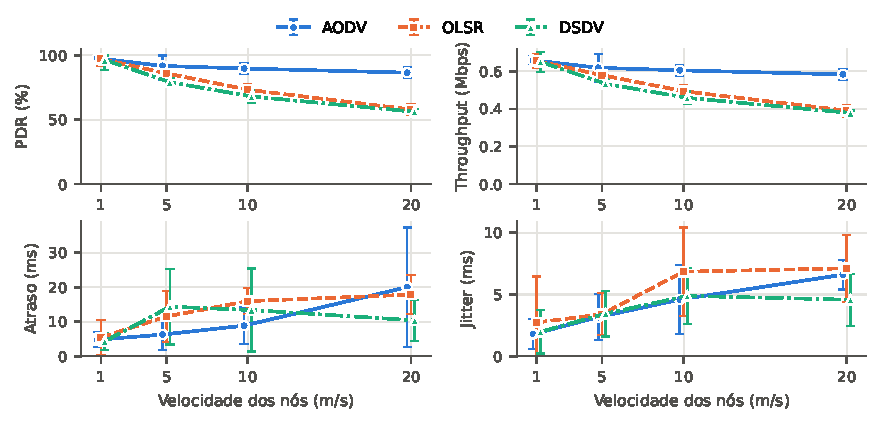
\includegraphics[width=\textwidth]{figuras/fig_base.pdf}
\caption{Métricas por velocidade (média de 10 execuções; barras: IC 95\%)}
\label{fig:base}
\end{figure}

\textbf{PDR e throughput.} A 1\,m/s os três protocolos empatam, com cerca de 96\% de
entrega (as diferenças pareadas incluem zero). Com a velocidade, o AODV perde 8,5 pontos
percentuais até 20\,m/s, e OLSR e DSDV perdem 37,7 e 38,2. A diferença pareada AODV$-$OLSR
é de 6,2 $\pm$ 5,4 p.p. a 5\,m/s, 17,1 $\pm$ 4,6 a 10\,m/s e 27,9 $\pm$ 4,3 a 20\,m/s
(Figura~\ref{fig:pareado}, à esquerda). Entre OLSR e DSDV só há diferença significativa a
5\,m/s. O throughput segue o PDR. Não há ruptura brusca: nos proativos a queda é mais
rápida até 10\,m/s (2 a 3,6 p.p. por m/s) e mais lenta depois (1,5).

\textbf{Explicação.} A diferença está no tempo para perceber que um enlace quebrou. O AODV
do ns-3 usa o aviso de falha da camada de enlace e refaz a rota em seguida. O OLSR descarta
um vizinho só após 6\,s sem HELLO; o DSDV anuncia tabelas a cada 15\,s. A 20\,m/s
um nó atravessa os 197\,m de alcance em cerca de 10\,s, tempo da ordem desses
temporizadores, e os proativos usam rotas que já não existem. O controle do AODV quase
dobra de 1 para 20\,m/s (11,4 para 22,0\,kbps), enquanto o de OLSR e DSDV cresce pouco; e
os pacotes que OLSR e DSDV entregam a 20\,m/s percorrem menos saltos (1,42 e 1,29, contra
1,70 no AODV), sinal de que as rotas longas são as que falham. O resultado
concorda com \cite{broch1998,johansson1999}.

\begin{figure}[ht]
\centering
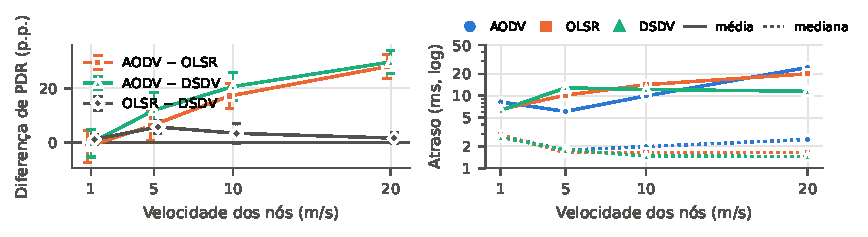
\includegraphics[width=\textwidth]{figuras/fig_pareado_atraso.pdf}
\caption{Esquerda: diferença de PDR entre protocolos no mesmo \emph{run} (IC 95\%).
Direita: média e mediana do atraso (escala logarítmica)}
\label{fig:pareado}
\end{figure}

\textbf{Atraso e jitter.} A média do atraso cresce com a velocidade (AODV de 8,2 para
24,5\,ms; OLSR de 6,5 para 20,0\,ms), mas a mediana fica entre 1,5 e 3\,ms em todos os
casos (Figura~\ref{fig:pareado}, à direita). A média é puxada por poucos pacotes que
esperam numa fila enquanto o protocolo procura outra rota: com 10 nós a 20\,m/s, o AODV
tem atraso médio de 99,5 $\pm$ 40,2\,ms e mediana de 1,5\,ms. Essa cauda explica a grande
variação da média e do jitter (de 2,8\,ms a 1\,m/s para 5 a 8\,ms a 20\,m/s, com
intervalos sobrepostos). Assim, a mobilidade é clara em PDR e throughput, aparece na cauda
do atraso e não muda o atraso típico.

A Figura~\ref{fig:comparativo} compara os protocolos a 20\,m/s, onde mais se separam.

\begin{figure}[ht]
\centering
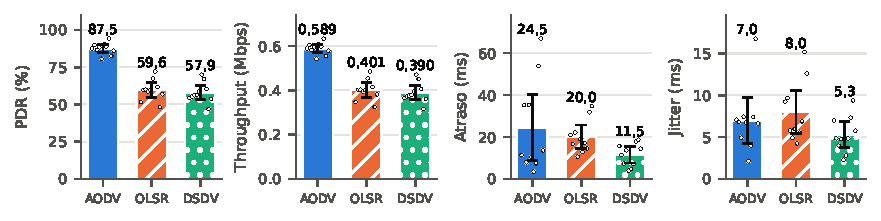
\includegraphics[width=\textwidth]{figuras/fig_comparativo.pdf}
\caption{Comparativo a 20\,m/s (barra: média; haste: IC 95\%; pontos: as 10 execuções)}
\label{fig:comparativo}
\end{figure}

\textbf{Variáveis adicionais.} A Figura~\ref{fig:extensao} mostra o PDR por velocidade
para cada quantidade de nós (em cima) e cada tempo de pausa (embaixo). O \textbf{tempo de
pausa} confirma que o fator é a mobilidade efetiva: a 20\,m/s, de 0 para 60\,s de pausa,
OLSR e DSDV sobem de 59,6\% e 57,9\% para 88,0\% e 85,6\%, o AODV de 87,5\% para 92,9\%, e
a diferença AODV$-$OLSR cai de 27,9 para 4,9 p.p. (o efeito aparece a partir de 30\,s). A \textbf{densidade} reduz a vantagem do AODV: a
20\,m/s com 40 nós ele entrega 75,3\%, contra 65,4\% do OLSR, e a 1\,m/s com 40 nós a ordem
se inverte (AODV 87,7\%, proativos acima de 96\%). O motivo é o custo da descoberta de
rotas por difusão: a 10\,m/s o controle do AODV passa de 15,5\,kbps com 20
nós para 103\,kbps com 40, contra 48\,kbps do OLSR. Com 10 nós a rede é esparsa e
varia mais.

\begin{figure}[ht]
\centering
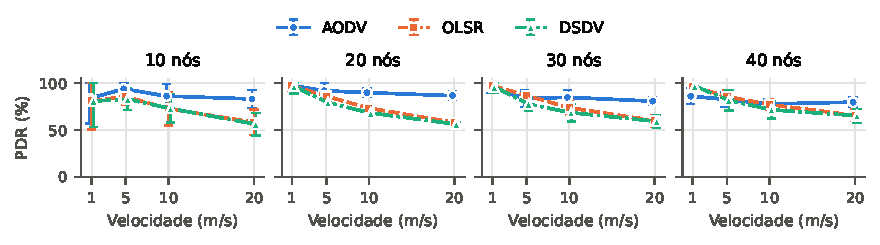
\includegraphics[width=\textwidth]{figuras/fig_extensao.pdf}
\caption{PDR por velocidade: em cima, 10 a 40 nós; embaixo, pausa de 0 a 60\,s (IC 95\%)}
\label{fig:extensao}
\end{figure}

\section{Conclusão}

A mobilidade reduz a entrega nos três protocolos, mas o reativo é bem menos afetado: a
20\,m/s o AODV entrega 87,5\%, contra 59,6\% do OLSR e 57,9\% do DSDV (diferença pareada de
28 a 30 p.p.); em baixa velocidade os três se equivalem. A mobilidade aumenta a média do
atraso e o jitter por poucos pacotes muito atrasados, sem mudar o atraso típico. Pausas
longas aproximam os protocolos, e redes densas encarecem a descoberta de rotas do AODV.

Essas conclusões valem para os parâmetros padrão do ns-3.48, dez repetições, espaço livre
e Random Waypoint, que concentra os nós no centro da área \cite{camp2002}. Trabalhos
futuros: ajustar os temporizadores dos proativos, aumentar a carga e testar outros modelos
de mobilidade e propagação.

\bibliographystyle{sbc}
\bibliography{referencias}

\end{document}
